\documentclass[letterpaper,10pt]{article}

\usepackage{titling}
\usepackage{listings}
\usepackage{url}
\usepackage{setspace}
\usepackage{subfig}
\usepackage{sectsty}
\usepackage{pdfpages}
\usepackage{colortbl}
\usepackage{multirow}
\usepackage{multicol}
\usepackage{relsize}
\usepackage{amsmath}
\usepackage{wasysym}
\usepackage{fancyvrb}
\usepackage{amssymb}
\usepackage{ifsym}
\usepackage{amsmath,amssymb,amsthm,graphicx,xspace}
\usepackage[titlenotnumbered,noend,noline]{algorithm2e}
\usepackage[compact]{titlesec}
\usepackage{XCharter}
\usepackage[T1]{fontenc}
\usepackage{tikz}
\usetikzlibrary{arrows,automata,shapes,trees,matrix,chains,scopes,positioning,calc}
\tikzstyle{block} = [rectangle, draw, fill=blue!20, 
    text width=2.5em, text centered, rounded corners, minimum height=2em]
\tikzstyle{bw} = [rectangle, draw, fill=blue!20, 
    text width=4em, text centered, rounded corners, minimum height=2em]

\definecolor{namerow}{cmyk}{.40,.40,.40,.40}
\definecolor{namecol}{cmyk}{.40,.40,.40,.40}

\let\LaTeXtitle\title
\renewcommand{\title}[1]{\LaTeXtitle{\textsf{#1}}}


\newcommand{\handout}[5]{
  \noindent
  \begin{center}
  \framebox{
    \vbox{
      \hbox to 5.78in { {\bf ECE356: Database Systems } \hfill #2 }
      \vspace{4mm}
      \hbox to 5.78in { {\Large \hfill #4  \hfill} }
      \vspace{2mm}
      \hbox to 5.78in { {\em #3 \hfill} }
    }
  }
  \end{center}
  \vspace*{4mm}
}

\newcommand{\lecture}[3]{\handout{#1}{#2}{#3}{Lecture #1}}
\newcommand{\tuple}[1]{\ensuremath{\left\langle #1 \right\rangle}\xspace}

\addtolength{\oddsidemargin}{-1.000in}
\addtolength{\evensidemargin}{-0.500in}
\addtolength{\textwidth}{2.0in}
\addtolength{\topmargin}{-1.000in}
\addtolength{\textheight}{1.75in}
\addtolength{\parskip}{\baselineskip}
\setlength{\parindent}{0in}
\renewcommand{\baselinestretch}{1.5}
\newcommand{\term}{Winter 2018}

\singlespace


\begin{document}

\lecture{ 17 --- Query Processing, Continued }{\term}{Jeff Zarnett}

\section*{Query Processing, Continued}

Having examined in some detail the idea of different strategies for carrying out a select operation. The next thing we would like to do is expand to more advanced queries, specifically, join queries. Join queries will be cripplingly inefficient if they operate on unsorted data. Remember that in a join, we need to match a tuple of the left hand relation with a tuple of the right hand relation. If for every tuple we had to linearly search the right hand relation, that would be painful. One way or another, we probably have to sort one of the relations to make this work.

\subsection*{Digression: Sorting}

So let us take a few minutes to talk about sorting. Wait, I hear you say, you already know ALL about sorting, insertion sort and selection sort and bogo sort and radix sort. Yes, also merge sort and quick sort. When you learn about sorting in a data structures and algorithms context, you are sorting a manageable amount of data. Manageable in the previous sentence means the full set of data can be fit into memory. For those, we can use all the standard algorithms. In the world of databases we need an algorithm that does not depend on loading everything into memory.

Sorting relations that do not fit into memory is called external sorting, and we will learn the external sort-merge algorithm from~\cite{dsc}. The basic plan works a lot like the merge sort algorithm works: divide the data into smaller units, sort the smaller units, then merge the smaller sorted units into a larger sorted unit. The sorting of each smaller unit will take place in memory, as per normal, and then we need to do an N-way merge where $N$ is the number of smaller units to be merged. Let's expand on this.

Step one of the algorithm is to divide the file into $N$ chunks of size $M$ where $M$ is the number of blocks that can fit into the area of memory available for sorting. Each chunk is as big as it can be for the constraints of the system, but no bigger. This chunk is called a \textit{run}. Each run $i$ is then sorted and it is written to a temporary file called $R_{i}$.

Step two of the algorithm now merges it. If $N$ is less than $M-1$ we have the simpler case and we can complete the merge in one pass. In that case we load the first block of $R_{i}$ for each $i$ from $0$ to $N-1$ into memory and we allocate an output block. Then we choose the first tuple from the all of the blocks, and move it into the output block. If a block $R_{i}$ becomes empty, replace it with the next block in that run (if there is one). If the output block becomes full, write it out and allocate a new output block. Continue this algorithm until all runs are empty. 

If $N$ is large enough that we cannot do it all in a single pass, we will do multiple passes. We will combine the first $M-1$ runs into a temporary file, and then the next (up to) $M-1$ runs, and so on, until the last run has been processed. Then we repeat the process using the larger runs as input until we produce the sorted file.

An example may help to clarify. Suppose the file consists of 10~000 blocks and we can fit 50 blocks in memory to do the sort. We can therefore create runs of 10~000/50 = 200 blocks each. Each run is sorted. Then we come to merge them. We cannot fit a block from each of the 200 runs inside the 49 available (50 - 1 block for output) so we must do multiple passes. The first pass sorts runs 1 through 49 into a new run (let's call it $R'_{1}$), then runs 50 - 98 into $R'_{2}$, et cetera, until the last one which is then 197-200 in $R'_{5}$. These larger $R'$ runs are then combined using the same merge procedure as before. Since there are only 5 we are sure the merge will complete in this second pass and we have the output file we wanted.

A visual representation of a two step sort merge from~\cite{dsc}:

\begin{center}
	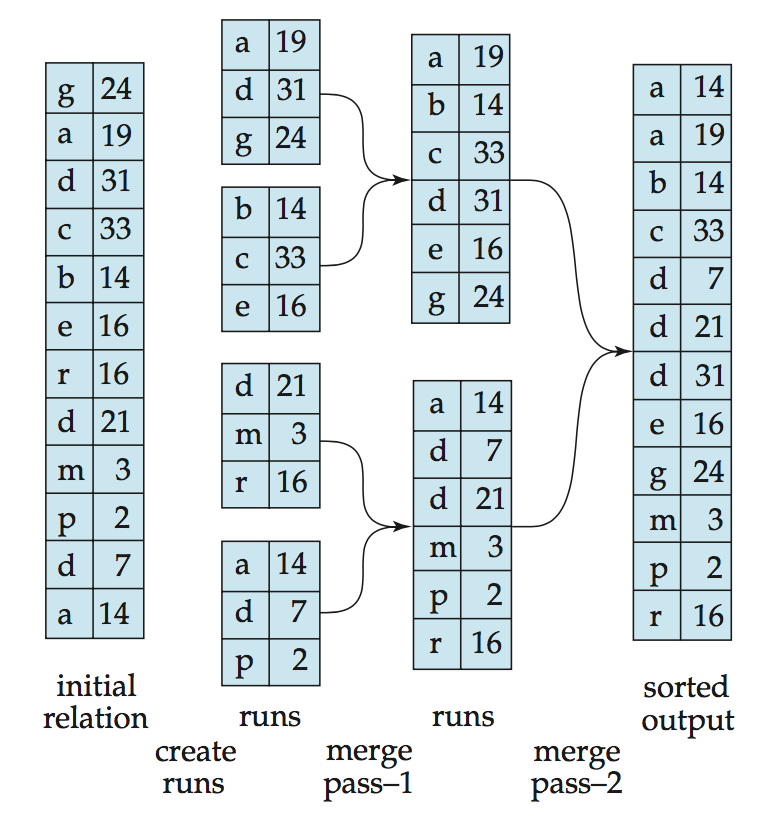
\includegraphics[width=0.5\textwidth]{images/external-merge}
\end{center}

Sorting has a cost, of course and the cost analysis also follows from~\cite{dsc}. If the number of blocks in the relation $r$ is $b_{r}$, the first step of the algorithm requires us to read in each block of the relation and write it out again for a cost of $2b_{r}$. The number of runs decreases by $M-1$ in each merge pass, so the number of merge passes is $\lceil log_{M-1}(b_{r}/M)\rceil$. Each pass reads reads every block of the relation and writes it once, except the last pass doesn't need to write the last output to disk as it is just going to send it on elsewhere. So the total number of block transfers is $b_{r}(2\lceil log_{M-1}(b_{r}/M)\rceil + 1)$. 

The total number of disk seeks is more complicated: If each run has $b_{b}$ blocks, then each merge pass requires $\lceil b_{r}/b_{b}\rceil$ seeks to read data. And we need to then write the output which costs  $2\lceil b_{r}/b_{b}\rceil$ for ever merge pass, except the last, since it gets sent on. So the total number of seeks is $2\lceil b_{r}/b_{b}\rceil + \lceil b_{r}/b_{b}\rceil(2 \lceil log_{M-1}(b_{r}/M)\rceil - 1)$.

What a fun equation that was! Referencing the two sep merge above, we get a total of 44 seeks: computed as $8 + 12 \times (2 \times 2 - 1)$ seeks if the value of $b_{b}$ is set at 1.

\subsection*{Join Operation}

There are several ways to compute a join, and we will analyze the costs of a few of the different approaches. Whatever route is actually taken, it's important to note that joins can be very expensive depending on how this is to be computed. The join we are looking to examine is the one introduced in relational algebra as $\Join_{\theta}$, specifically $r_{1} \Join_{r_{1}.a = r_{2}.b} r_{2}$ (or in SQL, an \texttt{INNER JOIN} with an explicit \texttt{ON} predicate). As before, the strategies described come from~\cite{dsc}.

\subsubsection*{Nested-Loop Joins}

The simple way to do a join is using one of the nested-loop strategies. It's called the nested loop strategy because that's exactly what it is: we have two nested for loops.

\paragraph{Join Strategy 1: Nested-Loop}
As with the select operation, the first option we are going to look at is basically a linear search and most likely has terrible performance characteristics. It is, however, a fallback option that we can always choose even if we can't choose anything else. This requires no index exist on either field $a$ or $b$ (the join attributes).

The algorithm described in pseudocode is:
\begin{verbatim}
1. for each tuple i in r1
2.   for each tuple j in r2
3.     if i.a equals j.b
4.       add (i join j) to the result
5.     end if
6.   end for
7. end for
\end{verbatim}

This is, after all, the brute force algorithm, so we expect that the number of tuples that needs to be examined is the number of tuples in $r_{1}$ (let's call it $n_{1}$) multiplied by the number of tuples in $r_{2}$ ($n_{2}$). In the best case scenario, both relations fit in memory at the same time and the cost is just two seeks plus a transfer for each of the blocks of $r_{1}$ (which we will call $b_{1}$) and a transfer for each of the blocks of $r_{2}$ ($b_{2}$). In the worst case we get only one block of each relation at a time. The inner loop then is one seek plus $b_{2}$ transfers to read it into memory. The outer loop requires one seek and one transfer for each block of $r_{1}$, plus one run of the inner loop for each tuple in $b_{1}$. So the total amount of seeks is $2 b_{1}$ and the number of blocks to be transferred is $b_{1} + n_{1} \times b_{2}$.

To illustrate with an example the difference between the best and worst case scenario, let us assign some numbers to $n_{1}$, $b_{1}$ and $b_{2}$. Suppose $n_{1}$ is 1600, $b_{1}$ is 100 blocks, $n_{2}$ is 10000, and $b_{2}$ is 500. Sticking with values used earlier, a seek takes 4~ms and a transfer 0.1~ms. In the best case scenario, the cost is 2 seeks plus a transfer for each block, or: $2 \times t_{s} + (b_{1} + b_{2}) \times t_{T} = 2 \times 4 + (100 + 500) \times 0.1 = 8 + 60 = 68$ ms. In the worst case scenario, the number of seeks is $2b_{1}$ plus the number of transfers as $b_{1} + n_{1} \times b_{2}$, or: $2 \times b_{1} \times t_{s} + (b_{1} + n_{1} \times b_{2}) \times t_{T} = 2 \times 100 \times 4 + (100 + 1600 \times 500) \times 0.1 = 200 \times 4 + 800000 \times 0.1 = 800 + 80000 = 80800$ ms. Yikes. That is a really huge difference. Conclusion: buy more RAM.

Assuming that $b_{1}$ is not equal to $b_{2}$ we can actually observe something interesting: it could be worse! The so-called worst case scenario is actually the second-worst case scenario. Imagine if the order of the relations is switched in the join loop). Let's do the math again: $2 \times b_{2} \times t_{s} + (b_{2} + n_{2} \times b_{1} \times t_{T} = 2 \times 500 \times 4 + (500 + 10000 \times 100) \times 0.1 = 1000 \times 4 + 1000500 \times 0.1 = 4000 + 100050 = 104050$ ms. So much worse. That's about 1.29 times more just based on the choice of which relation is $b_{1}$ and which is $b_{2}$.

Under this strategy it matters quite a lot which relation is the outer loop and which one is the inner loop. It would be vastly preferable to make the outer loop the smaller of the two relations since it minimizes the number of seeks as well as reduces the number of transfers. 

\paragraph{Join Strategy 2: Block Nested-Loop}
The previous strategy could be improved by thinking in terms of block operations rather than in terms of individual tuples. Instead of running the inner loop once for each tuple in the outer loop, we could run it once for each block in the other relation and that might be a lot less painful in terms of count of disk reads. Again, we are still assuming that no index is available, so we have to do this the ``hard'' way.

If everything fits in memory, then the block nested-loop strategy is really no improvement over the regular nested loop algorithm. It gains an advantage if there will be more memory reads. The primary improvement is that instead of loading the inner blocks once for every tuple of the outer relation, they are loaded once per block of the outer relation. Thus there are $b_{1} \times b_{2} + b_{1}$ transfers and $2\times b_{1}$ seeks that take place.

To once again use the same values as before, there are now $2 \times b_{1} = 2 \times 100 $ seeks which at a cost of 4 ms = $200 \times 4 = 800$ ms seek time, plus $b_{1} \times b_{2} + b_{1} = 100 \times 500 + 100 = 50100$ at a cost of 0.1 ms = $5010$ ms. Summed up a total of $5810$ ms to complete this.

As before it could be worse if we swapped the order of the relations. $2 \times b_{2} = 2 \times 500 $ seeks which at a cost of 4 ms = $1000 \times 4 = 4000$ ms seek time, plus $b_{2} \times b_{1} + b_{2} = 500 \times 100 + 500 = 50500$ at a cost of 0.1 ms = $5050$ ms. The total is then $9050$ ms which is about 1.56 times the cost of the other ordering. 

Of course, you may not lose sleep over this considering that the slower approach here is only 11\% of the cost of even the faster simple nested-loop approach. But why not choose the strategy that is 7\%? 

\paragraph{Join Strategy 3: Index Nested-Loop}
Suppose an index is available on one of the two relations. If so, then we don't have to do this in the most painful way; we can use the index instead. Since we will iterate over the inner relation more times, we want the index to be on the inner relation, if we have only one index to work with.

To find which tuples in the inner relation match the outer relation tuple $t_{1}.a$ then we do an index lookup on $r_{2}$ to find the tuple(s) that match. The worst case scenario will once again be that we can only get one block of the relation into memory. We will need to do one seek for each block of the outer relation $b_{1}$ and then one transfer for it. We will also need to, once for each tuple in $b_{1}$ look into the relation $r_{2}$. The formula is $b_{1} ( t_{s} + t_{T} ) + n_{1} \times c$  where $c$ is the cost of doing a single selection in that table using an index (if available). We already know everything we need to know about how to estimate $c$ since we already discussed four strategies for how to do a selection with an equality condition.

As before, the run time is faster if $n_{1}$ is the smaller value; that is, the outer relation should have fewer tuples. 

\subsubsection*{Merge Join}
The merge join might be more properly called the \textit{sort merge join} approach. Suppose relations $r_{1}$ and $r_{2}$ have some set of common attributes $r_{1} \cap r_{2}$ and we wish to compute the natural join. If both relations are sorted on  $r_{1} \cap r_{2}$ then we can do a merge-sort-like algorithm to compute the join.

\paragraph{Join Strategy 4: Merge-Join}
A description of the algorithm in pseudocode is in~\cite{dsc} but it it sensible to approach the concepts before looking at what is a long algorithm. The algorithm has one pointer for each relation, initialized to the first tuple in that relation. Then advance those pointers. Then each tuple of $r_{1}$ with the same value of the join attributes is read into a temporary block. Then the tuples of $r_{2}$ are read and processed as they go.

The aforementioned temporary block does need to be big enough to contain all the tuples of $r_{1}$ for each value of the join attributes. That is usually not a problem since we hope not too many tuples match that particular condition. If they do, we would expect either that (1) the database server has a lot of data and therefore needs a lot of RAM and can have the space to do this; or (2) the index is on an inappropriate field (e.g., boolean value) and we should not be trying to use this algorithm. The fallback plan is then the block nested-loop strategy.

Once again, the best case scenario is the two seeks plus reading in each block of each relation. In the worst case, we one seek for each block of the relation as well as a transfer for each block of each relation: $(b_{1} + b_{2})(t_{s} + t_{T})$.

There is also an assumption that the relations in question are sorted on the attributes of the join. While that may be true if one of them is a primary key attribute, it is probably not the case for the other relation. As you would imagine, a join of employees and departments relies on relations employee and department and it is unlikely that employees will be sorted based on department ID or vice versa. Each will have their own primary key. 

\paragraph{Join Strategy 5: Hybrid Merge-Join}

We can execute a variant of the merge-join approach on unsorted tuples if a secondary index exists on the join attribute(s). Normally if we are accessing the second relation through an index of some sort, we get the tuples in sorted order (from the view of that index), but they could be anywhere in the disk blocks meaning that each time we go to the next tuple is potentially another disk seek and transfer.

To save ourselves some work we can use the hybrid merge-join algorithm. The basic idea here is to merge the sorted relation $r_{1}$ with the leaf entries of $r_{2}$'s secondary index. The output is then made up of tuples of $r_{1}$ and pointers to the tuples of $r_{2}$. This file can then be sorted on the pointers to $r_{2}$ tuples so that accesses to $r_{2}$ go in physical storage order rather than jumping everywhere back and forth.

\paragraph{Join Strategy 6: Hash Join}
Another important strategy can be used for joining relations and it relies on hashing as we have already discussed. However, the complexity of the hash join is high and we will consider it beyond the scope of this course. Those who are curious can find more information in~\cite{dsc}.

\subsection*{Other Considerations in Query Processing}

There are a few more situations beyond the select and join scenarios that we will care about when we have to actually execute a query. Let us see a few more things from~\cite{dsc} that note some extra work we may have to do if the query is slightly more complex.

\paragraph{Distinct.} Often times in performing a query we are asked to remove duplicates (e.g., select distinct). This is easy enough if we are sorting the data because two identical values will be next to each other for merging. Alternatively, we could simply avoid writing them to the output at all if the sort-inserted routine finds something already in the designated space for that value. This can be expensive, so this is generally done only if we really ask for it.

\paragraph{Projection.} Projection should probably get a mention: it is pretty much just throwing away any columns of the relation that we don't need in some way. Projection could happen in several steps; if employee ID is used in a where condition, for example, but not asked for in the output, we might first project the full tuple down to the output fields plus those used in the where condition, then later throw away some more when presenting the final results. The same is true of an order-by clause: if that field is not needed in the output we will toss it out once the ordering is complete.

\paragraph{Set Operations.} Set operations (union, intersection, difference) are fairly self explanatory as well. Sorting the data is necessary, generally, to make this efficient. If there is no index, we might need to build one. Each relation $r_{x}$ is partitioned into different parts which we will label $r_{x_{0}}, r_{x_{1}}...$. A quick recap from~\cite{dsc} on how to do the various operations:

\begin{itemize}
	\item Union
	\begin{enumerate}
		\item Build an in memory hash index on the $r_{1_{i}}$
		\item Add the tuples $r_{2_{i}}$ to the index if they are not present
		\item Add the tuples referenced in the index to the result.
	\end{enumerate}
	
	\item Intersection
	\begin{enumerate}
		\item Build an in memory hash index on the $r_{1_{i}}$
		\item For each of the tuples in $r_{2_{i}}$, see if it is already in the index, and if so, add it to the output.
	\end{enumerate}
	
	\item Difference
	\begin{enumerate}
		\item Build an in memory hash index on the $r_{1_{i}}$
		\item For each of the tuples in $r_{2_{i}}$, see if it is already in the index, delete it from the index.
		\item Add the tuples referenced in the index to the result.
	\end{enumerate}

\end{itemize}

\paragraph{Outer Join.}
The outer join operation requires us to add some tuples that don't have a match in the other relation. A nested loop algorithm isn't too bad: if there is no match then pad the tuples with nulls on the appropriate side(s) and add it to the output. An alternative strategy is then to compute the (regular) join, then do a select on all tuples, subtracting those without a match, and pad those tuples and add them to the result.

\paragraph{Aggregation.} One approach to aggregation is more or less the same as the idea of duplicate removal. We select all the ones we need to aggregate, then take a second pass through the data to sort it, and then merge the values as are necessary. But this is probably not the best way, as might occur to you when thinking about count. Count might be done slightly more efficiently since we can skip the sort and merge entries part by simply keeping a running count. That might also be applied to min, max, sum if we are clever enough to maintain those values and update them accordingly. Average would require maintaining two values and then performing a division... but somehow this seems rather possible.

\paragraph{Order of Operations.} When dealing with simple expressions there is one operator and we have seen that it can sometimes matter in which order the operands occur. This problem of order of operations becomes larger when we start having complex queries. $r_{1} \bowtie r_{2} \bowtie r_{3}$ could be executed with two different groupings and with different orders of operands: 
\begin{enumerate}
\item $(r_{1} \bowtie r_{2}) \bowtie r_{3}$,  
\item $(r_{2} \bowtie r_{1}) \bowtie r_{3}$, 
\item $r_{3} \bowtie (r_{1} \bowtie r_{2})$,
\item $r_{3} \bowtie (r_{2} \bowtie r_{1})$,
\item $r_{1} \bowtie (r_{2} \bowtie r_{3})$. 
\item $r_{1} \bowtie (r_{3} \bowtie r_{2})$. 
\item $(r_{2} \bowtie r_{3}) \bowtie r_{1}$
\item $(r_{3} \bowtie r_{2}) \bowtie r_{1}$
\end{enumerate}

Sometimes we do not have quite this degree of freedom, however, and an order is necessarily implied, such as a subquery. In the next topics we will examine evaluations of expressions and look in more detail at how we decide which approach is likely to be best.

\bibliographystyle{alphaurl}
\bibliography{356}


\end{document}
